%%MO: changes other than compression
%% - changed notation for mean normalization in sect 5 to avoid confusion
%%   of two notions of mu
%% - moved tables out of the middle of paragraphs since that's visually
%%   easier for me to deal with in editing

\documentclass{kluwer}    % Specifies the document style.

\newdisplay{guess}{Conjecture}


\usepackage{graphicx}
\usepackage{qtree}

%\newcommand{\headlabel}[2]{\ensuremath{\underset{\textrm{#2}}{\textrm{#1}}}}
\newcommand{\headlabel}[2]{
  \begin{tabular}{c} #1\\
    {\small #2} \end{tabular}}
\newcommand{\arclabel}[1]{\ensuremath{\stackrel{#1}{\to}}}

\newcommand{\precision}[1]{\ensuremath{\textrm{Prec}\left(#1\right)}}
\newcommand{\recall}[1]{\ensuremath{\textrm{Recall}\left(#1\right)}}


\begin{document}
\begin{article}
\begin{opening}         
\title{Expected Dependency Pair Match:
Predicting translation quality with expected syntactic structure} 
\author{Jeremy G. \surname{Kahn}\email{jgk@u.washington.edu}}  
\institute{University of Washington}
\author{Matthew \surname{Snover}\email{snover@cs.umd.edu}}
\institute{University of Maryland}
\author{Mari \surname{Ostendorf}\email{ostendor@u.washington.edu}}  
\institute{University of Washington}
\runningauthor{Kahn, Snover \& Ostendorf}
\runningtitle{Expected Dependency Pair Match}
%s\date{May 10, 2009}

\begin{abstract}
  Recent efforts to develop new machine translation
  evaluation methods have tried to 
  account for allowable wording differences either in terms of
  syntactic structure or synonyms/paraphrases. This paper primarily considers syntactic structure, combining scores from partial syntactic dependency
  matches with standard local n-gram matches using a statistical
  parser, and taking advantage of N-best parse probabilities.  The new scoring metric, Expected Dependency
  Pair Match (EDPM), is shown to outperform BLEU and TER in terms
  of correlation to human judgments and as a predictor of HTER. Further, we combine the syntactic features of EDPM with the
  alternative wording features of TERp, showing a benefit to accounting for syntactic structure on top of
  semantic equivalency features.
\end{abstract}
\keywords{machine translation evaluation, syntax, dependency trees}

\end{opening}           

\section{Introduction}
\label{sec:intro}

A challenge in automatic machine translation (MT) evaluation is accounting
for allowable variability: two equally good
translations may be quite different in surface form. 
Currently, the most popular approaches are BLEU \cite{papineni02bleu},
based on $n$-gram precision, and Translation Edit Rate (TER), an
edit distance \cite{snover06ter}.
%evaluation measures include a measure
%based on $n$-gram precision known as BLEU \cite{papineni02bleu} and
%the edit-distance measure Translation Edit Rate (TER)
%\cite{snover06ter}.  
These measures can only account for variability when 
given multiple translations, and studies show that they may
not accurately track translation quality 
%both empirically
\cite{charniak03syntaxlmmt,callisonburch06bleuproblems} 
%and theoretically
%\cite{callisonburch06bleuproblems}.

Alternative measures that 
incorporate synonym knowledge sources include: METEOR
\cite{banerjee05meteor}, which uses synonym tables and
morphological stemming to do progressively more forgiving matching;
%%MO: I am taking out the tuning stuff here since it isn't critical
%It can be tuned towards recall or precision, but is generally not
%tuned by users.  
TER Plus (TERp) \cite{snover09terp}, which is an extension of the
previously-mentioned TER that also incorporates synonym sets and stemming, along
with automatically-derived paraphrase tables.  
%TERp is explicitly
%intended to be tuned to a development set by users.
%
%Tuning has the advantage that the weight of different types of errors
%can be adjusted to match the needs of the task, though it makes it
%more difficult to compare results across tasks, particularly when
%there is little data for tuning.
Other metrics modeling syntactically-local (rather than string-local)
word-sequences include: tree-local
$n$-gram precision in various configurations of constituency and
dependency trees \cite{liu05syntaxformteval};
%%MO: Since sparseval is cited elsewhere, I don't think we need the endnote
%\endnote{The dependency-based SParseval measure
%\cite{roark06:sparseval}, designed as a parse-quality metric for
%speech, is a similar approach, in that it is an F-measure over a
%decomposition of reference and hypothesis trees.} 
and the \textbf{d} and
\textbf{d\_var} measures proposed by \inlinecite{owczarzak07evaluatingmt}
%%MO: This is a hack to get the second year without the name
(2007b) 
that compare relational tuples derived from a
lexical functional grammar (LFG)
over reference and hypothesis translations.\endnote{
  \inlinecite{owczarzak07evaluatingmt} extend their previous line of
  research \cite{owczarzak07labelleddepseval}  by variably-weighting
%%MO: you actually do variable weighting using parse probabilities, so
%% would be good to mention what they use.  If you can say this in a few
%% words, then you won't add a line
  dependencies and by including synonym matching, two directions not
  pursued here. Hence, the earlier paper is cited in comparisons.
}
%
These syntactically-oriented measures require a system for proposing
dependency structure over the reference and hypothesis
translations. \inlinecite{liu05syntaxformteval} use a
PCFG parser with deterministic head-finding, while 
\cite{owczarzak07evaluatingmt} extract the semantic dependency
relations from an LFG parser \cite{cahill04lfg}.
%
This work extends the dependency-scoring strategies of
\inlinecite{owczarzak07evaluatingmt}, which reported substantial
improvement in correlation with human judgment relative to BLEU and
TER, by using a 
publicly-available probabilistic context-free grammar (PCFG) parser and deterministic head-finding rules. In addition, we consider more types of constituents and different score combinations, as well as combination with of synonym-type scores.
 
MT measures are evaluated in a variety of ways. Some
\cite{banerjee05meteor,liu05syntaxformteval,owczarzak07evaluatingmt}
comparing the measure to human
judgments of fluency and adequacy.  In other work, e.g.\
\cite{snover06ter}, measures are compared to
human-targeted TER (HTER), a distance to a human-revised reference
that uses wording closer to the MT system choices (keeping the
original meaning) that is intended to measure the post-editing work
required after translation.  In this paper, we explore both kinds of
evaluation.

We describe our approach to including syntax in MT
evaluation by outlining a family of metrics in
section~\ref{sec:approach} and implementation details in
section~\ref{sec:paradigm}.  Section~\ref{sec:faexpts} examines the
correlation of members of this family with human judgments of
fluency and adequacy, using the 
\cite{owczarzak07evaluatingmt} paradigm to provide comparisons and
select a best case configuration, Expected Dependency Pair Match
(EDPM). The EDPM measure is then compared to BLEU and TER in terms of
correlation with HTER, exploring language/genre effects in
section~\ref{sec:hter1} and combination with TERp's synonym/paraphrase
features in section~\ref{sec:hter2}. Finally, findings and future work
are summarized in section~\ref{sec:conclusion}.

\section{Approach}
\label{sec:approach}


The specific family of dependency pair match (DPM) measures explored here
combines precision and recall scores of various
decompositions of a syntactic dependency tree. These measures are
extensions of the dependency-pair F measures found in
\inlinecite{owczarzak07labelleddepseval}.  Rather than comparing
string sequences, as BLEU does with its $n$-gram precision, this
approach defers to a parser for an indication of the relevant word
tuples associated with meaning --- in these implementations, the head
on which that word depends.  Each sentence (both reference and
hypothesis) is converted to a labeled syntactic dependency tree and
then relations from each tree are extracted and compared.

We motivate the use of dependencies with actual translations:\\[4pt]
{\sl
Ref: Authorities have also closed southern Basra's airport and seaport.\\
S1: The authorities also closed the airport and seaport in the
southern port of Basra.\\
S2: Authorities closed the airport and the port of.\\[4pt]
}
A human judged the system 1 result (S1) as equivalent to the reference, but the system 2 (S2) result as
having errors.  BLEU gives both a similar score (0.199
vs.\ 0.203). TER scores S2 as better (errors
of 0.9 vs.  0.7, respectively), since a simple deletion requires fewer
edits that rephrasing.  By representing matches of dependencies, we
obtain a score for S1 from the new EDPM measure that is higher than
that for S2 (0.414 vs.\ 0.356).  The two phrases ``southern Basra's
airport and seaport'' and ``the airport and seaport in the southern
port of Basra'' have more in similarities in terms of dependencies
than word order.

The particular relations that are extracted from the dependency tree
are referred to here as \emph{decompositions}.
Figure~\ref{fig:decompexample}
illustrates the \emph{dependency-link-head} decomposition of a toy
dependency tree into a list of $\langle d, l, h \rangle$ tuples.  Some
members of the DPM family may apply more than one decomposition; other
good examples are the $dl$ decomposition, which generates a bag of
dependent words with outbound links, and the $lh$ decomposition, which
generates a bag of inbound link labels, with the head word for each
included. Figure~\ref{fig:decompexample2} shows the $dl$ and $lh$
decompositions for the same hypothesis tree.


\begin{figure}
  \centering
  \begin{tabular}{rcc}
    & \textbf{Reference} & \textbf{Hypothesis} \\
    \textbf{tree}
    & 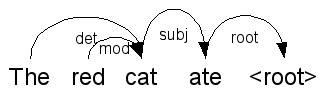
\includegraphics[scale=0.5]{dpm-example-ref} & 
    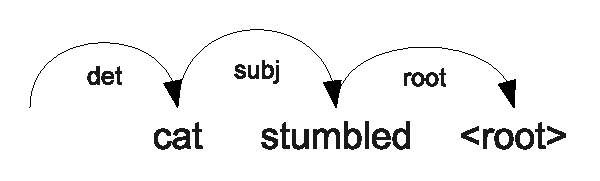
\includegraphics[scale=0.5]{dpm-example-hyp}\\
    \textbf{$dlh$ list} &
    \begin{tabular}{@{$\langle$}c@{,~}c@{,~}c@{$\rangle$}}
      the & \arclabel{\texttt{det}}  &  cat \\
      red & \arclabel{\texttt{mod}}  &  cat \\
      cat & \arclabel{\texttt{subj}} &  ate \\
      ate & \arclabel{\texttt{root}} &  $<$root$>$ \\
    \end{tabular} & 
    \begin{tabular}{@{$\langle$}c@{,~}c@{,~}c@{$\rangle$}}
      the &      \arclabel{\texttt{det}}  &  cat \\
      cat &      \arclabel{\texttt{subj}} &  stumbled \\
      stumbled & \arclabel{\texttt{root}} &  $<$root$>$ \\
    \end{tabular}\\
  \end{tabular}\\
%%MO: I don't think we need the P/R/F at this point in the narrative
%  Precision$_{dlh}$ is $\frac{1}{3}$ and Recall$_{dlh}$ is
%  $\frac{1}{4}$: thus $F[dlh] = \frac{2}{7}$
  \caption{Example dependency trees and their $dlh$ decompositions.}
  \label{fig:decompexample}
\end{figure}

\begin{figure}
  \centering
    \begin{tabular}{cc}
    $dl$ & $lh$ \\
    \hline
    \begin{tabular}{@{$\langle$}c@{,~}c@{$\rangle$}}
      the & \arclabel{\texttt{det}}  \\
      cat & \arclabel{\texttt{subj}} \\
      stumbled & \arclabel{\texttt{root}} \\
    \end{tabular} &
    \begin{tabular}{@{$\langle$}c@{,~}c@{$\rangle$}}
      \arclabel{\texttt{det} } &  cat \\
      \arclabel{\texttt{subj}} &  stumbled \\
      \arclabel{\texttt{root}} &  $<$root$>$ \\
    \end{tabular}\\
  \end{tabular}
  \caption{The $dl$ and $lh$ decompositions of the hypothesis tree in
    figure~\ref{fig:decompexample}.
%     $\precision{dl} = \frac{2}{3}$,
%     $\recall{dl} = \frac{2}{4}$, $\precision{lh} = \frac{2}{3}$,
%     $\recall{lh} = \frac{2}{4}$, so $F[dl,lh] = \frac{4}{7}$
  }
  \label{fig:decompexample2}
\end{figure}

It is worth noting here that the $dlh$ and $lh$ decompositions (but
not the $dl$ decomposition) ``overweight'' the headwords, in that
there are $n$ elements in the resulting bag, but if a word has no
dependents it is found in the resulting bag exactly one time (in the
$dlh$ case) or not at all (in the $lh$ case).  Conversely,
syntactically ``key'' words, that are directly modified by many other
words in the tree, are included multiple times in the decomposition
(once for each inbound link).  This ``overweighting'' leverages
syntactic indications of which words are more
important to translate correctly (e.g., ``Basra'' in the
example).

A statistical parser provides confidences associated with parses
in an $n$-best list, which we use to compute
expected counts for each decomposition in both reference and
hypothesized translations. The expected counts lead to partial matches
(or weighted counts) used in computing precision and recall.
This approach addresses both error
in the best parse and ambiguity in the translations (reference and
hypothesis).

% Reviewer 2 suggests reducing/removing the use of \mu here to a basic
% explanation.

%%MO: I think that it is important to keep because of some of the comparisons
%% you make, so I will try to just compress

When multiple decomposition types are used together, we may combine
these subscores in a variety of ways. Here, we experiment with using
two variations of a harmonic mean:
computing precision and recall over all
decompositions as a group (giving a single precision and recall number)
vs.\ computing precision and recall separately for each decomposition.
We distinguish between these using the notation:
\begin{eqnarray}
  \label{eq:fprmeans}
  F[dl,lh] & = &
  \mu_h \left( \precision{dl \cup lh},
    \recall{dl \cup lh} \right) \\
  \mu_{PR}[dl,lh]  & = & \mu_h \left( \precision{dl},
    \recall{dl}, \precision{lh}, \recall{lh} \right)    
\end{eqnarray}
where $\mu_h$ represents a harmonic mean.
Dependency-based SParseval \inlinecite{roark06:sparseval} 
and the \textbf{d} approach from
\inlinecite{owczarzak07evaluatingmt} may each be understood as
$F[dlh]$, while the latter's \textbf{d\_var} method may be understood
as something close to $F[dl,lh]$.
%
Both the combination methods $F$ and
$\mu_{PR}$ are ``naive'' in that they treat each component
score as equivalent to the next.  When we introduce syntactic/paraphrasing
features, we will move to a weighted combination.

%%MO: actually the next section does more than this, and this sentence is
%% essentially repeated later, so I deleted it here
%The possible family of metrics outlined above is quite large. In the
%next section, we make explicit the range of these parameters that we
%explore in this article.

%%MO: I changed the title, since I usually put corpus in ``paradigm''. You 
%% are really just talking about implementation here

\section{Parsing and dependency extraction}
\label{sec:paradigm}

The family of DPM measures may be implemented with
any parser that generates a dependency graph (a single labelled arc
for each word, pointing to its head-word). Prior work
\cite{owczarzak07evaluatingmt} on related
measures has used an LFG parser \cite{cahill04lfg} or
an unlabelled dependency tree \cite{liu05syntaxformteval}. 

In this work, we use a state-of-the-art PCFG (the first stage of
\inlinecite{charniak-johnson:2005:ACL}) and context-free head-finding
rules \cite{magerman95headfinding} to generate an N-best list of
dependency trees for each hypothesis and reference translation.  We
use the parser's default (English) Wall Street Journal
training parameters.  Head-finding uses the Charniak parser's rules,
with three modifications to make the semantic (rather than syntactic)
relations more dominant in the dependency tree: prepositional and
complementizer phrases choose nominal and verbal heads respectively
(rather than functional heads) and auxiliary verbs are modifiers of
main verbs (rather than the converse). These changes capture the
fact that main verbs are more important for adequacy in translation, as
illustrated by the functional equivalence of ``have also closed'' vs.\ 
``also closed'' in the example in section~\ref{sec:approach}.

Having constructed the dependency tree, we label the arc between dependent
$d$ and its head $h$ as $A/B$ when $A$ is the lowest constituent-label
headed by $h$ and dominating $d$ and $B$ is the highest constituent
label headed by $d$).
%
For example, in figure~\ref{fig:depextract}, the S node is the lowest
node headed by \emph{stumbled} that dominates \emph{cat}, and the NP
node is the highest constituent label headed by \emph{cat}, so the arc
linking \emph{cat} to \emph{stumbled} is labelled $S/NP$.
%
This strategy is very similar to one adopted in the reference
implementation of labelled-dependency \textsc{SParseval} \cite{roark06:sparseval}, and may be
considered as a shallow approximation of the rich semantics generated by LFG
parsers \cite{cahill04lfg}.
%
The $A/B$ labels are not as descriptive as the LFG semantics, but they
have a similar resolution, e.g.\ the $S/NP$ arc label
usually represents a subject dependent of a sentential verb.

\begin{figure}
  \Tree
  [.\headlabel{S}{stumbled}
    [.\headlabel{NP}{cat}
      [.\headlabel{DT}{the} the ]
      [.\headlabel{NN}{cat} cat ]
    ]
    [.\headlabel{VP}{stumbled} 
      [.\headlabel{VBD}{\it stumbled} stumbled ]
    ]
  ]
  \\
  \begin{center}
    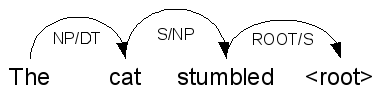
\includegraphics[scale=0.6]{dpm-example-depextract}
  \end{center}
  \caption{An example constituent tree (heads of each constituent are
    listed below the label) and the labelled dependency tree
    derived from it.}
  \label{fig:depextract}
\end{figure}

%%MO: I added this though reviewers didn't ask for it, since I thought that
%% this is actually a tricky concept plus the flattening description should
%% really go here. You might want to change the example
For the cases where we have N-best parse hypotheses, we use the associated
parse probabilities (or confidences) to compute expected
counts. The sentence will then be represented with more tuples,
corresponding to alternative analyses. For example, if the N-best
parses include two different roles for dependent ``Basra'', then two
different $dl$ tuples are included, each with the weighted count that is the
sum of the confidences of all parses having the respective role.\endnote{
    The use of expectations with N-best parses is different from 
    \textbf{d\_50} and \textbf{d\_50\_pm} in \cite{owczarzak07evaluatingmt}
    in that the latter uses the best-matching pair of trees rather than an 
    aggregate over the tree sets and they do not use parse
    confidences.}
The parse confidence $\tilde{p}$ is normalized so that the
N-best confidences sum to one. Because the parser is overconfident, we
explore a flattened estimate: $\tilde{p}(k) =
\frac{p(k)^\gamma}{\sum_ip(i)^\gamma},$ where $k,i$ index the parse and
$\gamma$ is a free parameter.

%%MO: I took this out, since this is not true now that you have more info
%The uniform distribution ($\gamma = 0$) is equivalent to the \cite{owczarzak07evaluatingmt}
%  \textbf{d\_50} and \textbf{d\_50\_pm} measures.

\section{Correlation with human judgments of fluency \& adequacy}
\label{sec:faexpts}

We explore various configurations of the DPM by assessing the results
against a corpus of human judgments of fluency and adequacy,
specifically the LDC Multiple Translation Chinese corpus parts
2~\cite{LDC03MTC2} and 4~\cite{LDC06MTC4}, which are composed of
translations of written Chinese news stories.  These corpora include
multiple human judgments of fluency and adequacy for each sentence
(assigned on a five-point scale), with each judgment using a different
human judge and a different reference translation.  For a
rough\endnote{Our segment count differs slightly from
  \inlinecite{owczarzak07evaluatingmt}
  for the same corpus: 16,807 vs.\ 16,815. 
  As a result, the baseline 
  per-segment correlations differ slightly (BLEU$_4$ is higher here,
  while TER here is lower), but the trends in gains over those
  baselines are very similar.  } comparison with
\inlinecite{owczarzak07evaluatingmt}, we treat each judgment as a
separate segment, which yields 16,815 tuples of $\langle$hypothesis,
reference, fluency, adequacy$\rangle$.  We compute per-segment
correlations.\endnote{The use of the same hypothesis translations in
  multiple comparisons in the Multiple Translation Corpus means that
  scored segments are not strictly independent, but for methodological
  comparison with prior work, this strategy is preserved.}
%
The baselines for comparison are case-sensitive BLEU (4-grams, with add-one smoothing) and TER. 

The specific dimensions of DPM explored include:
\begin{description}
\item[Decompositions.] We compute precision and recall of:
  \begin{description}
  \item[dlh] $\left\langle \textrm{Dependent}, \textrm{arc Label},
      \textrm{Head}\right\rangle$ -- full triple
  \item[dl] $\left\langle \textrm{Dependent}, \textrm{arc Label}
      \right\rangle$ --  marks how the word
      fits into its syntactic context (what it modifies)
    \item[lh] $\left\langle \textrm{arc Label}, \textrm{Head}
      \right\rangle$ --  implicitly marks how
      key the word is to the sentence
    \item[dh] $\left\langle \textrm{Dependent}, \textrm{Head}
      \right\rangle$ -- drops syntactic-role information.
    \item[1g,2g] -- simple measures of unigram
      (bigram) precision and recall.
  \end{description}
\item[Parser variations.] When using more than one parse, we explore:
  \begin{description}
  \item[Size of $n$-best list.] 50 (as in \cite{owczarzak07evaluatingmt})
  \item[Parse confidence.] The distribution flattening
    parameter is varied from $\gamma=0$ (uniform distribution) to $\gamma=1$
    (no flattening).
%%MO: I recall that you tried more than one possible gamma in the middle
%% range to get the 0.25 value, so I think it is misleading to say you looked
%% at 3 cases.
  \end{description}
\item[Score combination.] Global $F$ vs.\ component harmonic mean $\mu_{PR}$.
\end{description}


Considering only the 1-best parse, we compare DPM with different
decompositions to the baseline measures.
Table~\ref{tab:facorr:subgraphs} shows that all decompositions except
$[dlh]$ have a better per-segment correlation with the
fluency/adequacy scores than TER or BLEU$_4$. Dependencies $[dl,lh]$
and string-local n-grams $[1g,2g]$ give similar results, but the
combination gives further improvement.  The results also confirm, with
a PCFG, what \inlinecite{owczarzak07evaluatingmt} found with an LFG
parser: that partial-dependency matches are better correlated with
human judgments than full-dependency links. Including progressively
larger chunks of the dependency graph with $F[1g,dl,dlh]$, inspired by
the BLEU$_k$ idea of progressively larger $n$-grams, did not give an
improvement over $[dl,lh]$.  $F$ gives substantially better results than
$\mu_{PR}$, which is never better than BLEU for these decompositions.

\begin{table}
  \caption{Per-segment correlation with
    human fluency/adequacy judgments of baselines and different decompositions.}
  \label{tab:facorr:subgraphs}
  \begin{tabular*}{2.5in}{lr}
    \hline
    metric  &    \multicolumn{1}{c}{$|r|$} \\
    \hline
    $F[1g,2g,dl,lh]$      &  0.237 \\
    $F[1g,2g]$            & 0.227 \\
    $F[dl,lh]$ &   0.226 \\
    % # +1 smoothing
    BLEU$_4$ &   0.218 \\
    $F[dlh]$ &     0.185 \\
    TER &      0.173 \\
    \hline
  \end{tabular*}
\end{table}

%In table~\ref{tab:facorr:combinations}, we compare combination methods
%for different decompositions, finding that $F$ consistently outperforms
%$\mu_{PR}$ as well as the BLEU basedline (from table~\ref{tab:facorr:subgraphs})$\mu_{PR}$ measures are never better than BLEU.  

% \begin{table}
%  \begin{tabular*}{2.5in}{lr}
%    \hline
%    metric  &    \multicolumn{1}{$r$} \\
%    \hline
%    $F[1g,2g,dl,lh]$      &  0.237 \\
%    $\mu_{PR}[1g,2g,dl,lh]$ &  0.217 \\
%    \rlcline{1-1} \rlcline{2-2}
%    $F[1g,2g]$            & 0.227 \\
%    $\mu_{PR}[1g,2g]$            & 0.215 \\
%    $F[1g,dl,dlh]$        & 0.227 \\
%    \rlcline{1-1} \rlcline{2-2}
%    $F[dl,lh]$            &  0.226 \\
%    $\mu_{PR}[dl,lh]$      &  0.208 \\
%    \hline
%  \end{tabular*}
%  \caption{Per-segment correlation with human fluency/adequacy judgments of different combination methods and decompositions.}
%  \label{tab:facorr:combinations}
%\end{table}

Table~\ref{tab:facorr:multiparse} shows the impact of using N-best
parses for different decompositions.
For the $n=50$ cases, we set $\gamma=0$ to assign uniform
probabilities, which was slightly better than $\gamma=1$.
%%MO: I want to take this out, since it really isn't a comparison
%% if they are using the best match.  I recalled that 0 was better than 
%% 1 -- change if not
%to compare as closely as possible
%to \inlinecite{owczarzak07evaluatingmt}, which includes a
%\textbf{d\_var\_50} measure with 50-best parses, with ranks but no
%weights.  
While not all of these differences are significant, there is a
consistent trend of correlation $r$ improving with 50 vs. 1 parse.  Tuning
experiments find that increasing $\gamma$ to 0.25 can increase the $r$
reported here for $F[1g,2g,dl,lh]$ (but insignificantly).

 \begin{table}
  \begin{tabular*}{2.5in}{lrr}
    \hline
    metric  & \multicolumn{1}{c}{$n$} &  \multicolumn{1}{c}{$r$} \\
    \hline
    $F[1g,2g,dl,lh]$      & 50 &  0.239 \\
    $F[1g,2g,dl,lh]$      &  1 &  0.237 \\
    \rlcline{1-2}\rlcline{3-3}
    $F[1g,dl,lh]$            &  50 & 0.237 \\
    $F[1g, dl,lh]$            &  1 & 0.234 \\
    \rlcline{1-2}\rlcline{3-3}
    $F[dl,lh]$            &  50 & 0.234 \\
    $F[dl,lh]$            &  1 & 0.226 \\
    \hline
  \end{tabular*}
  \caption{Per-segment correlation with human fluency/adequacy judgments
  comparing $n=1$ vs.\ 50 parses for different decompositions.}
  \label{tab:facorr:multiparse}
\end{table}

In summary, exploring a number of
variants of the DPM metric against an average fluency/adequacy
judgment leads to a best-case of:
\begin{displaymath}
  \mbox{EDPM} = F[1g,2g,dl,lh], n=50, \gamma=0.25
\end{displaymath}
We use this configuration in experiments assessing correlations with HTER.


\section{Correlating EDPM with HTER}
\label{sec:hter1}
In this section, we compare EDPM to baseline metrics in terms of
document- and segment-level correlation with HTER scores using the
GALE 2.5 translation corpus.  The corpus includes system translations
into English from three sites, all of which use system combination to
integrate results from several systems, some phrase-based and some
that use syntax on either the source or target side. No system
provided system-generated parses.
%
The source data comprises Arabic and Chinese in four
genres: \texttt{bc} (broadcast conversation), \texttt{bn} (broadcast
news), \texttt{nw} (newswire), and \texttt{wb} (web text), with corpus
sizes shown in table~\ref{tab:galestats}.
The corpus includes one English reference translation
\cite{gale08phase2_5references} for each sentence and a system
translation for each of the three systems. Additionally,
each of the system translations has a
corresponding human-targeted reference aligned at the sentence level,
so we have available the HTER score at
both the sentence and document level.

\begin{table}
  \begin{tabular}{r|rr|rr|rr}
    \hline
     & \multicolumn{2}{c|}{Arabic} & \multicolumn{2}{c|}{Chinese}
     & \multicolumn{2}{c}{Total}\\
     & doc & sent & doc & sent & doc   & sent\\
     \hline
     \texttt{bc}    & 59  & 750 & 56 & 1061 & 115 & 1811\\
     \texttt{bn}    & 63  & 666 & 63 & 620  & 126 & 1286\\
     \texttt{nw}    & 68  & 494 & 70 & 440  & 138 & 934 \\
     \texttt{wb}    & 69  & 683 & 68 & 588  & 137 & 1271\\
     \hline
     Total & 259 & 2593& 257& 2709 & 516 & 5302\\
     \hline
  \end{tabular}
  \caption{Corpus statistics for the GALE 2.5 translation
    corpus.}
  \label{tab:galestats}
\end{table}

HTER and automatic scores all degrade on average for more difficult sentences.
Since there are multiple system translations in this corpus, it is possible to 
roughly factor out this source of variability by correlating mean normalized
scores,\endnote{Previous work 
  \cite{kahn08metricsmatr} reported HTER
  correlations against pairwise differences among translations
  derived from the same source to factor out 
  sentence difficulty, but this violates
  independence assumptions used in the Pearson's $r$ tests.}
$\overline{m}(t_i) = m(t_i) - \frac{1}{I}\sum_{j=1}^Im(t_j)$
%\begin{equation}
%  \label{eq:meansub}
%  \overline{m}(t_i) = m(t_i) - \sum_{j=1}^I\frac{m(t_j)}{I}
%\end{equation}
where $m$ can be HTER, TER, BLEU or EDPM and $t_i$
represents the $i$-th translation of segment $t$.
Mean-removal ensures
that the reported correlations are among differences in the
translations rather than among differences in the underlying segments.

In table~\ref{tab:hterperdoc}, we show per-document Pearson's $r$
between $\overline{\textrm{EDPM}}$ and $\overline{\textrm{HTER}}$, as well as the $\overline{\textrm{TER}}$ and $\overline{\textrm{BLEU}}$$_4$
baselines. EDPM has the highest correlation in each of the
subcorpora created by dividing by genre or by source language, as well
as the corpus as a whole.   In structured data
(\texttt{bn} and \texttt{nw}), these differences are not always
significant, but in the unstructured domains (\texttt{wb} and
\texttt{bc}), EDPM is always significantly better than at least one of
the comparison baselines.

\begin{subtable}
  \begin{table}
    \begin{tabular}{r|rrrr|rr|r}
      \hline
      $r$ vs. $\overline{\textrm{HTER}}$ & \multicolumn{1}{c}{\texttt{bc}}
      & \multicolumn{1}{c}{\texttt{bn}} &
      \multicolumn{1}{c}{\texttt{nw}} & \multicolumn{1}{c}{\texttt{wb}}
      & \multicolumn{1}{|c}{all Arabic} & \multicolumn{1}{c|}{all Chinese}
      & \multicolumn{1}{c}{all} \\
      \hline
      $\overline{\textrm{TER}}$
      &  0.59 &  \textbf{0.35} &  \textbf{0.47}&  \textit{0.17}
      & \textbf{0.54} & \textbf{0.32} &  0.44\\
      $\overline{\textrm{BLEU}}$
      & -0.42 & \textbf{-0.32} & \textbf{-0.46}&  \textbf{-0.27}
      & -0.42  &  \textbf{-0.33} & -0.37 \\
      $\overline{\textrm{EDPM}}$
      & \textbf{-0.69} & \textbf{-0.39} & \textbf{-0.47} &
      \textbf{-0.27}
      & \textbf{-0.60} & \textbf{-0.39} & \textbf{-0.50} \\
      \hline
    \end{tabular}
    \caption{Per-document correlations of $\overline{\textrm{EDPM}}$ and others to
      $\overline{\textrm{HTER}}$, by genre and by source language. Bold numbers are
      within 95\% significance of the best per column; italics indicate
      that the sign of the $r$ value has less than 95\% confidence.}
    \label{tab:hterperdoc}
  \end{table}
  \begin{table}
    \begin{tabular}{r|rrrr|rr|r}
      \hline
      $r$ vs. $\overline{\textrm{HTER}}$ & \multicolumn{1}{c}{\texttt{bc}}
      & \multicolumn{1}{c}{\texttt{bn}} &
      \multicolumn{1}{c}{\texttt{nw}} & \multicolumn{1}{c}{\texttt{wb}}
      & \multicolumn{1}{|c}{all Arabic} & \multicolumn{1}{c|}{all Chinese}
      & \multicolumn{1}{c}{all} \\
      \hline
      $\overline{\textrm{TER}}$
      &  \textbf{0.44} &  \textbf{0.29} &  \textbf{0.33}&  0.25
      & \textbf{0.44} & 0.25  &  \textbf{0.36}\\
      $\overline{\textrm{BLEU}}$
      & -0.31 & -0.24  & -0.29 &  -0.25
      & -0.31  &  -0.24  & -0.28 \\
      $\overline{\textrm{EDPM}}$
      & \textbf{-0.46} & \textbf{-0.31} & \textbf{-0.34} &
      \textbf{-0.30}
      & \textbf{-0.44} & \textbf{-0.30} & \textbf{-0.37} \\
      \hline
    \end{tabular}
    \caption{Per-sentence, length-weighted correlations of
      $\overline{\textrm{EDPM}}$ and others to $\overline{\textrm{HTER}}$, by genre and by
      source language. Bold numbers indicate significance as above.}
    \label{tab:hterpersent}
  \end{table}
\end{subtable}


Table~\ref{tab:hterpersent} presents per-sentence correlations based on
scores normalized by sentence length in order to get a per-word measure which
reduces variance across sentences.  (Even with length weighting, the
$r$ values are smaller magnitude due to the higher variability at the
sentence level.)  EDPM again has the largest correlation in each
category, but TER has $r$ values within 95\%
confidence of EDPM scores on nearly every breakdown.

\section{Combining syntax, edit and semantic knowledge sources}
\label{sec:hter2}

While our results show that EDPM is as good or better than other
measures, the correlation is still low, which is consistent with
the example in section~\ref{sec:approach}, where the EDPM score is much less than 1 for the good
translation. For that
reason, we investigated combining the alternative wording features of
TERp with the EDPM syntactic features.

The TERp tools \cite{snover09terp} provide an optimizer for
weighting multiple simple subscores.  The TERp optimizer performs a
hill-climbing search, with randomized restarts, to maximize the
correlation of a linear combination of the subscores with a set of
human judgments.  Within the TERp framework the subscores are the
counts of the various edit types normalized for the length of the
reference, where the counts are determined after aligning the MT
output to the reference using default edit costs.

The experiments here leverage the TERp optimizer but extend
the set of subscores by including the syntactic and n-gram overlap
features (modified to reflect false and missed detection rates for the TERp
format rather than precision and recall). The subscores explored include:
\begin{description}
\item[E]: the 8 fully syntactic subscores from the EDPM family, including
  false/miss error rates for the $dl$, $lh$, $dlh$, and $dh$ decompositions. 
\item[N]: the 4 n-gram subscores from the DPM family;
  specifically, error rates for the $1g$ and $2g$ decompositions.
\item[T]: the 11 subscores from TERp, which include matches, insertions, deletions, substitutions, shifts, and
  synonym and stem matches, edit distances between paraphrases, and the. 
\end{description}

For these experiments, we again use the GALE 2.5 data, but with 2-fold
cross-validation in order to have independent tuning and test data.
Documents are partitioned randomly, such that each subset has the same
document distribution across source-language and genre. The objective
is length-normalized per-sentence correlation with HTER, using
mean-removed scores as before. In figure~\ref{fig:tuneresults}, we
plot the Pearson's $r$ (with 95\% confidence interval) for the results
on the two test sets combined, after linearly normalizing the
predicted scores to account for magnitude differences in the learned
weight vectors.  The baseline scores, which involve no tuning, are not
normalized.

\begin{figure}
  \begin{center}
    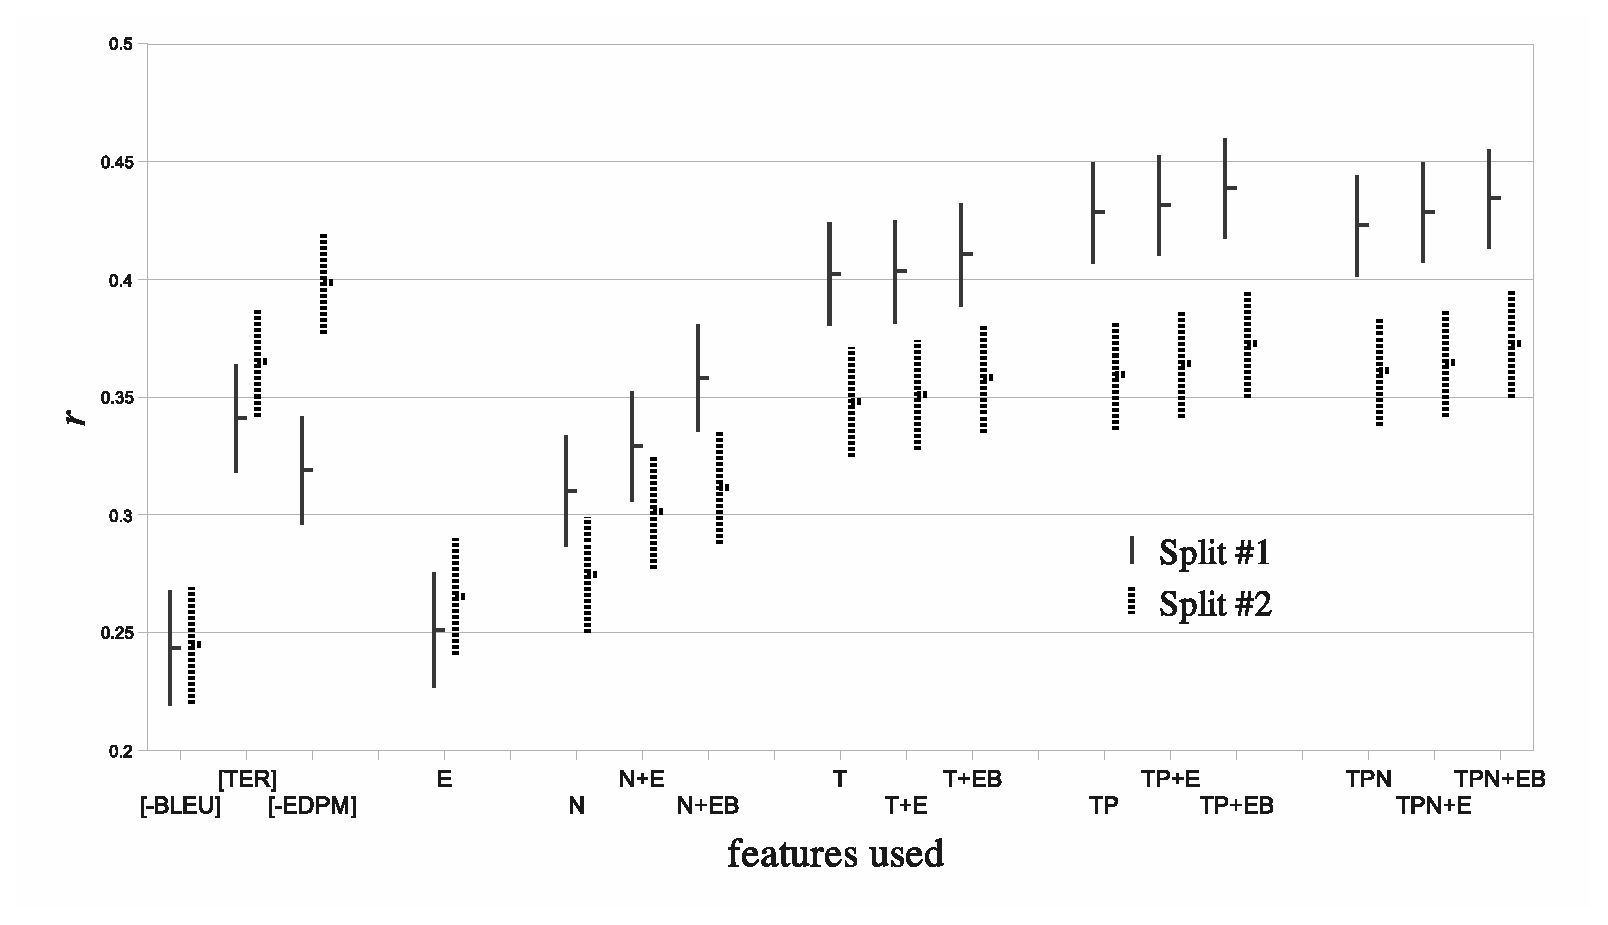
\includegraphics[scale=0.45]{tuning}
  \end{center}
  \caption{Pearson's $r$ for various feature tunings, with 95\%
    confidence intervals.}
  \label{fig:tuneresults}
\end{figure}

The figure shows that TER and EDPM are significantly more correlated with HTER than BLEU, consistent with the overall results of the previous section. The N+E combination outperforms E alone (i.e.\ it is helpful to use both n-gram and dependency overlap) but gives lower performance than EDPM because of the particular combination technique. Both findings are consistent with the fluency/adequacy experiments. The TERp features, which account for synonym/paraphrase differences, have much higher correlation with HTER than the syntactic E+N subscores.  However, a significant additional improvement is obtained by adding syntactic features to TERp (T+E). Adding the n-gram features to TERp (T+N) gives almost as much improvement, probably because most dependencies are local.  There is no further gain from using all three subscore types.

\section{Conclusion}
\label{sec:conclusion}
In summary, we explore a family of dependency pair match measures.  Through a corpus of human fluency
and adequacy judgments,
we settle on EDPM, a member of that family with promising predictive
power.  We find that EDPM is superior to BLEU and TER in terms of
correlation with human judgments and as a per-document and
per-sentence predictor of mean-normalized HTER.
We also experiment with including syntactic and synonym/paraphrase 
features in a TERp-style linear combination, and find that the combination
improves correlation with HTER over either method alone.

One difference with respect to the work of \inlinecite{owczarzak07evaluatingmt} is the use of a PCFG vs.\ an LFG parser. The PCFG has the advantage that it
is publicly available and easily adaptable to new domains.  However, the performance varies depending on the amount of labeled data for the domain, which raises the question of how sensitive EDPM and related measures are to parser quality.

A limitation of this method for MT system tuning is the computational
cost of parsing compared to word-based measures such as BLEU or TER.
Two alternative low-cost use scenarios include late-pass
evaluation, for choosing between different system architectures,
or system diagnostics, looking at
relative quality of these component scores compared to those of an
alternative configuration.

%%MO: put back if room,
%Another possible approach is to store packed forests
%\cite{huang08packedforests} rather than generating an $n$-best list
%only to sum across it again in calculating the expectation.

% \appendix
% [don't think we want an appendix]

\acknowledgements

{\small This material is based on work supported by the National
  Science Foundation under Grant No. 0741585 and the Defense Advanced
  Research Projects Agency under Contract Nos. HR0011-06-C-0022 and
  HR0011-06-C-0023.
% Re: DARPA contract numbers
% -0022 is Matt's [Agile] grant.
% -0023 is Mari & Jeremy's [Nightingale] grant
%%MO: slight rewording to save lines
  Any opinions, findings, conclusions or recommendations expressed
  herein are those of the authors and do not necessarily
  reflect the views of the funding agencies.  }

% The endnotes section will be placed here.  But I don't think we have any

\theendnotes

\bibliographystyle{klunamed}
\bibliography{mtjournal}

\end{article}
\end{document}